\chapter{Implementation and Evaluation}
\begin{center}
\large \textbf{A Rust Implementation of ML-KEM}
\end{center}
\vspace{1em}

The preceding chapters introduced the KEM abstraction and traced its technical development from KEM/DEM composition to ML-KEM. This chapter presents the implementation component of the project. The implementation, named \texttt{jkem}, is a teaching-oriented Rust implementation of ML-KEM following FIPS 203~\cite{nist2024fips203}. It supports the standard ML-KEM-512, ML-KEM-768, and ML-KEM-1024 parameter sets, and it is used in this report to study the concrete engineering interface between the algebraic K-PKE core, the Fujisaki-Okamoto style transform, and side-channel-aware implementation techniques. The source code is available at \url{https://github.com/wsm25/jkem}, and the generated documentation is available at \url{https://wsm.moe/jkem/jkem/}.

\section{Implementation Design}

\subsection{Implementation Goal and Scope}

The implementation has three main objectives. First, it aims to conform to the standard behavior of ML-KEM, as verified by deterministic Known Answer Tests (KATs) for keys, ciphertexts, and shared secrets. Second, it separates polynomial arithmetic, sampling, K-PKE algorithms, and ML-KEM control logic into distinct modules, making the correspondence between the specification and the code explicit. Third, it provides sufficient performance for empirical evaluation against an optimized baseline, while retaining a portable Rust implementation without architecture-specific assembly optimizations.

The public API exposes a generic type \texttt{MlKem<P>} parameterized by an ML-KEM parameter set, together with convenience aliases \texttt{MlKem512}, \texttt{MlKem768}, and \texttt{MlKem1024}. The three public operations follow the KEM syntax:
$$
\texttt{keygen()} \to (\texttt{ek}, \texttt{dk}), \qquad
\texttt{encaps(ek)} \to (\texttt{ct}, K), \qquad
\texttt{decaps(dk, ct)} \to K .
$$
Here \texttt{ek} is the encapsulation key, \texttt{dk} is the decapsulation key, \texttt{ct} is the ciphertext, and $K$ is the 32-byte shared secret.

\subsection{Dependencies and References}

The implementation uses a limited dependency set. The \texttt{getrandom} crate supplies operating-system randomness for public key-generation and encapsulation APIs. The \texttt{sha3} crate supplies SHA3 and SHAKE functions required by ML-KEM, including SHA3-256, SHA3-512, SHAKE128, and SHAKE256. The \texttt{subtle} crate is used for constant-time equality checks and conditional selection in decapsulation. The \texttt{zeroize} crate wipes selected temporary secret byte buffers. The \texttt{hybrid-array} crate provides fixed-size arrays indexed by type-level parameter sizes, which makes the same generic implementation cover all standard ML-KEM parameter sets.

The primary specification reference is FIPS 203~\cite{nist2024fips203}. We also use the Kyber/ML-KEM design lineage~\cite{bos2018crystals} to interpret the relationship between the module-lattice PKE core and the final CCA-secure KEM interface. The implementation is structured around the algorithms and byte layouts specified by the standard, rather than around the organization of any single reference implementation. Deterministic KAT files used for validation were obtained from \href{https://gist.github.com/itzmeanjan/c8f5bc9640d0f0bdd2437dfe364d7710}{Github Gist}.

\subsection{Architecture}

The implementation hierarchy follows the organization of FIPS 203~\cite{nist2024fips203}. The standard first specifies auxiliary algorithms, then the K-PKE component scheme, then the deterministic internal ML-KEM algorithms, and finally the public ML-KEM interface. The codebase preserves this ordering: each layer depends on the layers below it and exposes only the interface needed by the next layer.

\begin{enumerate}
    \item \textbf{Parameter-set layer.} Corresponding to FIPS 203 Section 8, the \texttt{params} module defines $n,q,k,\eta_1,\eta_2,d_u,d_v$ and the derived byte lengths for each approved parameter set. These definitions determine the dimensions of vectors, matrices, keys, and ciphertexts at compile time.
    \item \textbf{Auxiliary-algorithm layer.} Corresponding to FIPS 203 Section 4, the \texttt{math}, \texttt{security}, and serialization code implement the algorithms that are reused by the higher-level procedures. This layer includes arithmetic in
    $$
    R_q = \mathbb{Z}_q[X]/(X^{256}+1), \qquad q = 3329,
    $$
    polynomial and vector operations, the NTT and inverse NTT, byte encoding/decoding, compression/decompression, SHA3/SHAKE-based functions, matrix sampling, and centered binomial sampling.
    \item \textbf{K-PKE component layer.} Corresponding to FIPS 203 Section 5, the \texttt{kpke} module implements \texttt{K-PKE.KeyGen}, \texttt{K-PKE.Encrypt}, and \texttt{K-PKE.Decrypt}. This layer is the algebraic public-key encryption component used internally by ML-KEM.
    \item \textbf{Internal ML-KEM layer.} Corresponding to FIPS 203 Section 6, the \texttt{control} module and the internal methods \texttt{keygen\_internal}, \texttt{encaps\_internal}, and the deterministic core of \texttt{decaps} implement \texttt{ML-KEM.KeyGen\_internal}, \texttt{ML-KEM.Encaps\_internal}, and \texttt{ML-KEM.Decaps\_internal}. This layer performs key packing, public-key hash binding, derivation of shared secrets and encryption coins, re-encryption validation, and implicit rejection.
    \item \textbf{Public ML-KEM layer.} Corresponding to FIPS 203 Section 7, the generic type \texttt{MlKem<P>} exposes \texttt{keygen}, \texttt{encaps}, and \texttt{decaps}. This layer obtains randomness for public key generation and encapsulation, and invokes the deterministic internal layer.
\end{enumerate}

This hierarchy is important because FIPS 203 distinguishes deterministic internal algorithms from the randomized public KEM interface. In particular, \texttt{ML-KEM.KeyGen\_internal}, \texttt{ML-KEM.Encaps\_internal}, and \texttt{ML-KEM.Decaps\_internal} are deterministic once their inputs are fixed, whereas the public \texttt{ML-KEM.KeyGen} and \texttt{ML-KEM.Encaps} algorithms generate fresh randomness before calling the internal algorithms. The same separation is reflected in the implementation and is also used by the KAT tests.

\section{Implementation Details}

\subsection{Implementation of the ML-KEM Algorithms}

The theoretical role of KEM/DEM composition has been discussed in Chapter 3. This section therefore focuses on the FIPS 203 algorithm hierarchy as realized by the implementation.

\textbf{Key generation.} The public \texttt{keygen} API implements \texttt{ML-KEM.KeyGen}: it draws two 32-byte random values $d$ and $z$, then calls the deterministic internal algorithm. The internal algorithm first invokes \texttt{K-PKE.KeyGen}. In FIPS 203, this K-PKE procedure expands $d$ into $\rho$, used for public matrix sampling, and $\sigma$, used for secret noise sampling. In the implementation, this expansion is factored into the control layer before calling the K-PKE arithmetic routine, but the resulting $\rho,\sigma$ data flow is the same. The K-PKE component samples the public matrix in the NTT domain, samples the secret and error vectors, and computes the public-key polynomial vector. The ML-KEM internal layer then sets $\texttt{ek}=\texttt{ekPKE}$ and packs the decapsulation key as
$$
\texttt{dk} = \texttt{dkPKE} \parallel \texttt{ek} \parallel H(\texttt{ek}) \parallel z ,
$$
where $z$ is the secret fallback value used for implicit rejection.

\textbf{Encapsulation.} The public \texttt{encaps} API implements \texttt{ML-KEM.Encaps}: it draws a fresh 32-byte value $m$, then calls \texttt{ML-KEM.Encaps\_internal}. The internal algorithm computes
$$
(K, r) = G(m \parallel H(\texttt{ek})),
$$
where $K$ is the shared secret and $r$ is the deterministic encryption coins. It then invokes \texttt{K-PKE.Encrypt} with $\texttt{ek}$, $m$, and $r$. The K-PKE component regenerates the public matrix from $\rho$, samples the encryption noise from $r$, computes the ciphertext components, compresses and serializes them, and returns the ciphertext. The public API returns this ciphertext together with $K$.

\textbf{Decapsulation.} The public \texttt{decaps} API implements \texttt{ML-KEM.Decaps}. Since FIPS 203 specifies decapsulation as deterministic, this API does not draw randomness. It parses the ML-KEM decapsulation key into $\texttt{dkPKE}$, $\texttt{ek}$, $h=H(\texttt{ek})$, and $z$. The K-PKE component decrypts the ciphertext to recover a candidate message $m'$. The internal ML-KEM layer derives $(K',r')=G(m'\parallel h)$, computes the fallback secret $J(z\parallel\texttt{ct})$, and invokes \texttt{K-PKE.Encrypt} to re-encrypt $m'$ using $r'$. The re-encrypted ciphertext is compared with the received ciphertext to determine whether decapsulation follows the success path or the implicit-rejection path.

The final selection implements the Fujisaki-Okamoto style implicit rejection step. For a valid ciphertext, decapsulation returns the derived success secret. For an invalid ciphertext, it returns
$$
J(z \parallel \texttt{ct}),
$$
implemented with SHAKE256. This design avoids exposing ciphertext validity through an explicit failure return. In the implementation, the success secret and fallback secret are selected byte-by-byte using constant-time conditional selection from \texttt{subtle}.

\subsection{Parameter Abstraction}

The standard parameter sets are represented by marker types implementing a common parameter trait. This trait fixes the module rank $k$, noise parameters $\eta_1,\eta_2$, compression parameters $d_u,d_v$, and the resulting byte lengths for keys and ciphertexts. The three standard instances are summarized in Table~\ref{tab:ml-kem-parameters}.

\begin{table}[htbp]
    \centering
    \caption{ML-KEM standard parameter sets.}
    \label{tab:ml-kem-parameters}
    \begin{tabular}{c c c c c c}
        \toprule
        \textbf{Parameter set} & \textbf{$k$} & \textbf{$\eta_1$} & \textbf{$\eta_2$} & \textbf{$d_u$} & \textbf{$d_v$} \\
        \midrule
        ML-KEM-512  & 2 & 3 & 2 & 10 & 4 \\
        ML-KEM-768  & 3 & 2 & 2 & 10 & 4 \\
        ML-KEM-1024 & 4 & 2 & 2 & 11 & 5 \\
        \bottomrule
    \end{tabular}
\end{table}

Since the algorithms are generic over this trait, most implementation code is shared across all three parameter sets. The benchmark code additionally defines a non-standard experimental $k=5$ instance to evaluate whether the structure extends beyond the standardized choices. This instance is used only as an engineering extensibility experiment and is not a proposed cryptographic parameter set.

\subsection{Security Engineering Considerations}

The security engineering layer is intended to preserve the security semantics of ML-KEM in the executable implementation. Randomness is generated only at the public API boundary: key generation obtains $d$ and $z$, and encapsulation obtains $m$, from the operating-system random source. Deterministic internal hooks are therefore reserved for KAT reproduction and timing measurements. During decapsulation, the implementation computes both the candidate shared secret and the implicit-rejection fallback secret, compares ciphertexts with constant-time equality, and uses constant-time conditional selection for the returned secret. Selected secret byte buffers are also zeroed after use.

These measures should be understood as engineering precautions rather than as a formal constant-time proof or production security audit.

\section{Evaluation}

\subsection{Testing}

Correctness is tested against deterministic KAT files for ML-KEM-512, ML-KEM-768, and ML-KEM-1024. For each parameter set, the tests verify that the KAT file is present and unchanged, then check generated public keys, generated decapsulation keys, generated ciphertexts, encapsulated shared secrets, and decapsulated shared secrets. Each file contributes 100 test cases. The tests are included in the public codebase, so the reported results can be reproduced by running \texttt{cargo test} from the project root.

\begin{table}[htbp]
    \centering
    \caption{KAT integration test matrix.}
    \label{tab:kat-matrix}
    \begin{tabular}{c c c c c c c c}
        \toprule
        \textbf{Parameter set} &
        \textbf{File} &
        \textbf{PK} &
        \textbf{SK} &
        \textbf{CT} &
        \textbf{Enc SS} &
        \textbf{Dec SS} &
        \textbf{Malformed} \\
        \midrule
        ML-KEM-512  & \checkmark & \checkmark & \checkmark & \checkmark & \checkmark & \checkmark & \checkmark \\
        ML-KEM-768  & \checkmark & \checkmark & \checkmark & \checkmark & \checkmark & \checkmark & \checkmark \\
        ML-KEM-1024 & \checkmark & \checkmark & \checkmark & \checkmark & \checkmark & \checkmark & \checkmark \\
        \bottomrule
    \end{tabular}
\end{table}

The tests also cover malformed-input behavior. Modified ciphertexts do not produce explicit validity failures; instead, decapsulation returns the implicit rejection secret $J(z \parallel \texttt{ct})$. Malformed encapsulation keys with invalid encoded coefficients are rejected, and decapsulation keys with an incorrect stored $H(\texttt{ek})$ are rejected. The integration test suite contains 21 tests across the three parameter sets.

\subsection{Benchmark Methodology}

The benchmark evaluates the three public KEM operations: key generation, encapsulation, and decapsulation. Each operation is measured repeatedly and reported as time per operation, together with a normalized throughput estimate. The comparison baseline is \texttt{mlkem-native}, an optimized implementation with native low-level routines. This comparison highlights the performance cost of the portable generic Rust implementation relative to an implementation engineered primarily for high throughput.

\begin{table}[htbp]
    \centering
    \caption{Mean benchmark throughput in operations per second.}
    \label{tab:mlkem-benchmark}
    \begin{tabular}{l c c c}
        \toprule
        \textbf{Case} &
        \textbf{Key generation} &
        \textbf{Encapsulation} &
        \textbf{Decapsulation} \\
        \midrule
        \texttt{native/mlkem512}  & $40984$ & $34400$ & $27078$ \\
        \texttt{native/mlkem768}  & $25967$ & $21820$ & $17803$ \\
        \texttt{native/mlkem1024} & $16978$ & $14986$ & $12541$ \\
        \texttt{jkem/mlkem512}    & $9867$  & $7867$  & $5371$ \\
        \texttt{jkem/mlkem768}    & $5844$  & $4980$  & $3531$ \\
        \texttt{jkem/mlkem1024}   & $3799$  & $3365$  & $2485$ \\
        \bottomrule
    \end{tabular}
\end{table}

\begin{figure}[htbp]
    \centering
    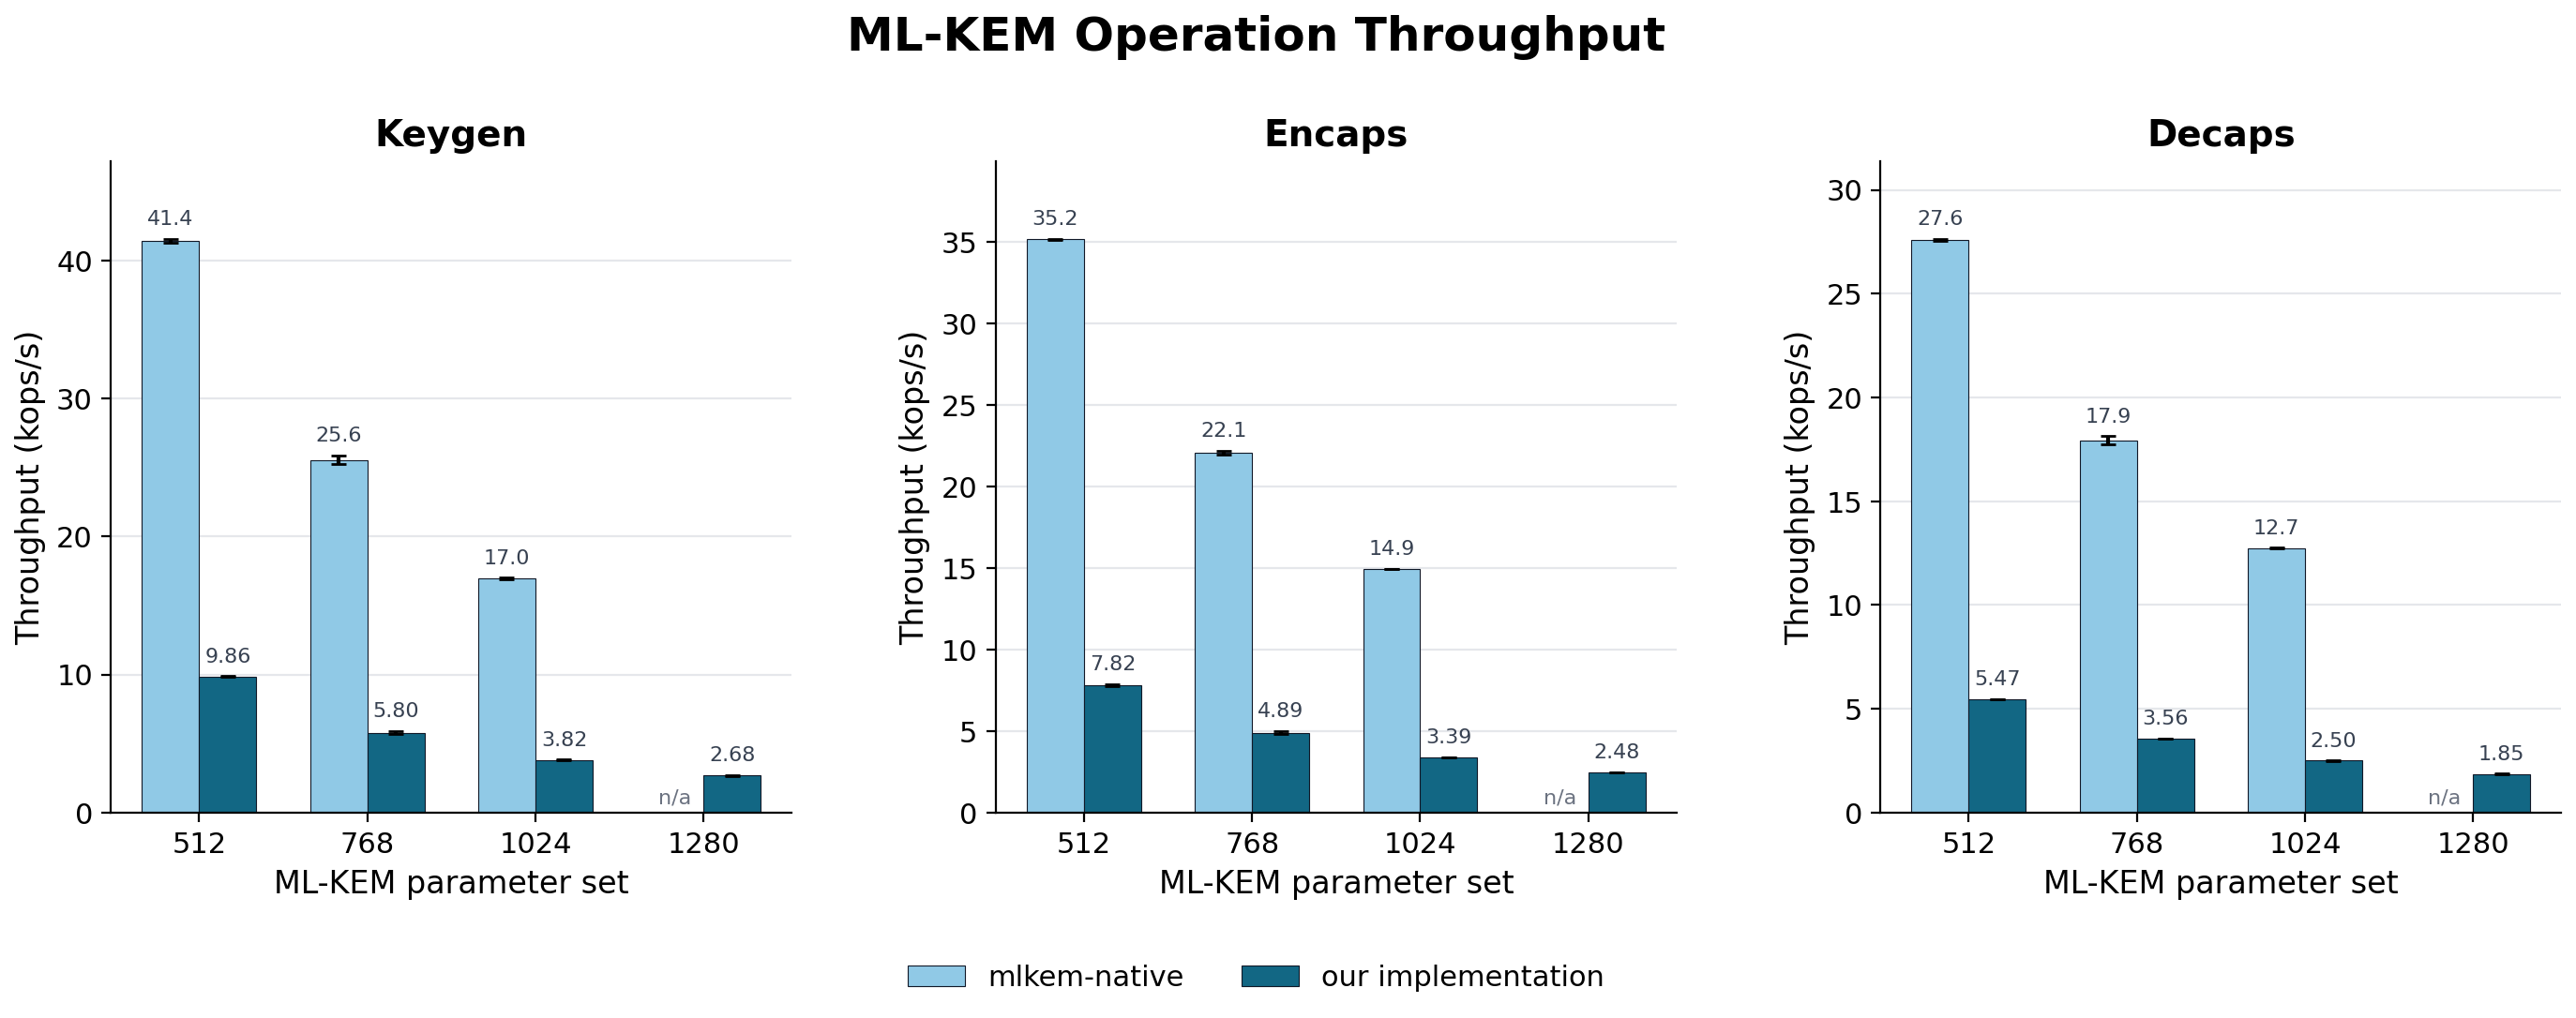
\includegraphics[width=1\textwidth]{images/mlkem-throughput-kops-s.png}
    \caption{Operation throughput for key generation, encapsulation, and decapsulation.}
    \label{fig:mlkem-kops}
\end{figure}

The throughput measurements in Table~\ref{tab:mlkem-benchmark} show a clear performance gap. Across the three standard parameter sets, the Rust implementation is slower than the optimized native baseline while preserving a simpler and more inspectable structure.

The benchmark suite also includes two traditional key-exchange baselines using OpenSSL: X25519 and finite-field Diffie-Hellman with the \texttt{modp2048-256} group. These benchmarks are not operation-for-operation equivalent to a KEM, because DH-style key exchange is symmetric while a KEM has separate encapsulation and decapsulation roles. A useful comparison is therefore the local work done by each endpoint in one unauthenticated key-establishment run. For DH, each endpoint performs one ephemeral key generation and one shared secret derivation. For ML-KEM-512, the encapsulating endpoint performs encapsulation, while the decapsulating endpoint performs key generation and decapsulation.

\begin{table}[htbp]
    \centering
    \caption{Endpoint CPU time for one key-establishment run.}
    \label{tab:kx-endpoint-time}
    \begin{tabular}{l c c c}
        \toprule
        \textbf{Case} &
        \textbf{Endpoint A} &
        \textbf{Endpoint B} &
        \textbf{Total local CPU time} \\
        \midrule
        \texttt{jkem/mlkem512} &
        $287.53\,\mu s$ &
        $127.11\,\mu s$ &
        $414.65\,\mu s$ \\
        \texttt{native/mlkem512} &
        $61.33\,\mu s$ &
        $29.07\,\mu s$ &
        $90.40\,\mu s$ \\
        \texttt{openssl/x25519} &
        $108.87\,\mu s$ &
        $108.87\,\mu s$ &
        $217.75\,\mu s$ \\
        \texttt{openssl/modp2048-256} &
        $1236.71\,\mu s$ &
        $1236.71\,\mu s$ &
        $2473.42\,\mu s$ \\
        \bottomrule
    \end{tabular}
\end{table}

Table~\ref{tab:kx-endpoint-time} shows that the portable Rust ML-KEM-512 implementation is slower than OpenSSL X25519 when both endpoints' local work is added together: about $414.65\,\mu s$ versus $217.75\,\mu s$, or roughly $1.90\times$ the CPU time. The split is asymmetric: the encapsulating side alone is close to one X25519 endpoint, while the key-generation and decapsulation side is more expensive. Against traditional finite-field Diffie-Hellman at the \texttt{modp2048-256} group, even this portable ML-KEM-512 implementation is substantially faster; its total local CPU time is about $0.17\times$ that of the two DH endpoints. The optimized \texttt{mlkem-native} ML-KEM-512 baseline is faster than both DH baselines in this measurement.

To estimate operation bandwidth, public key and ciphertext byte lengths are not a stable measure of the internal work done by ML-KEM, because the dominant algebraic work scales with the module rank $k$. To relate the measured operation throughput to $k$, we derive an approximate internal-data throughput. Let $N=256$ be the number of coefficients in one polynomial and let $s_c=2$ bytes be the in-memory size of one coefficient. One polynomial therefore accounts for
$$
B_{\mathrm{poly}} = N s_c = 512 \ \mathrm{bytes}.
$$

The normalization estimates the amount of polynomial data touched by the dominant algebraic operations. The $k^2$ term represents matrix generation and matrix-vector multiplication. The linear terms represent vector NTTs, inverse NTTs, noise polynomials, encoding/decoding, and additional dot products. The constant term accounts for the single-polynomial message or ciphertext component. Thus,
$$
\begin{aligned}
D_{\mathrm{keygen}}(k) &= B_{\mathrm{poly}}(k^2 + 4k),\\
D_{\mathrm{encaps}}(k) &= B_{\mathrm{poly}}(k^2 + 5k + 1),\\
D_{\mathrm{decaps}}(k) &= B_{\mathrm{poly}}(k^2 + 6k + 1).
\end{aligned}
$$
For an operation with measured time $t_{\mathrm{op}}(k)$ seconds, the normalized throughput is
$$
\operatorname{MB/s}_{\mathrm{real}}(\mathrm{op}, k) = \frac{D_{\mathrm{op}}(k)}{10^6 t_{\mathrm{op}}(k)} .
$$
Equivalently, if the benchmark reports $Q_{\mathrm{op}}(k)$ operations per second, then
$$
\operatorname{MB/s}_{\mathrm{real}}(\mathrm{op}, k) = \frac{D_{\mathrm{op}}(k) Q_{\mathrm{op}}(k)}{10^6}.
$$
This model is a first-order approximation: it does not separately weight fixed overhead, rejection sampling, SHA3/SHAKE setup, compression widths, or decapsulation's validation re-encryption. It is nevertheless sufficient to compare how throughput scales with $k$.

\begin{table}[htbp]
    \centering
    \caption{Normalized internal-data throughput derived from Table~\ref{tab:mlkem-benchmark}.}
    \label{tab:normalized-throughput}
    \begin{tabular}{l c c c}
        \toprule
        \textbf{Case} &
        \textbf{Key generation} &
        \textbf{Encapsulation} &
        \textbf{Decapsulation} \\
        \midrule
        \texttt{native/mlkem512}  & $251.81$ & $264.19$ & $235.69$ \\
        \texttt{native/mlkem768}  & $279.20$ & $279.30$ & $255.22$ \\
        \texttt{native/mlkem1024} & $278.17$ & $283.89$ & $263.26$ \\
        \texttt{jkem/mlkem512}    & $60.62$  & $60.42$  & $46.75$ \\
        \texttt{jkem/mlkem768}    & $62.83$  & $63.74$  & $50.62$ \\
        \texttt{jkem/mlkem1024}   & $62.24$  & $63.75$  & $52.17$ \\
        \bottomrule
    \end{tabular}
\end{table}

\begin{figure}[htbp]
    \centering
    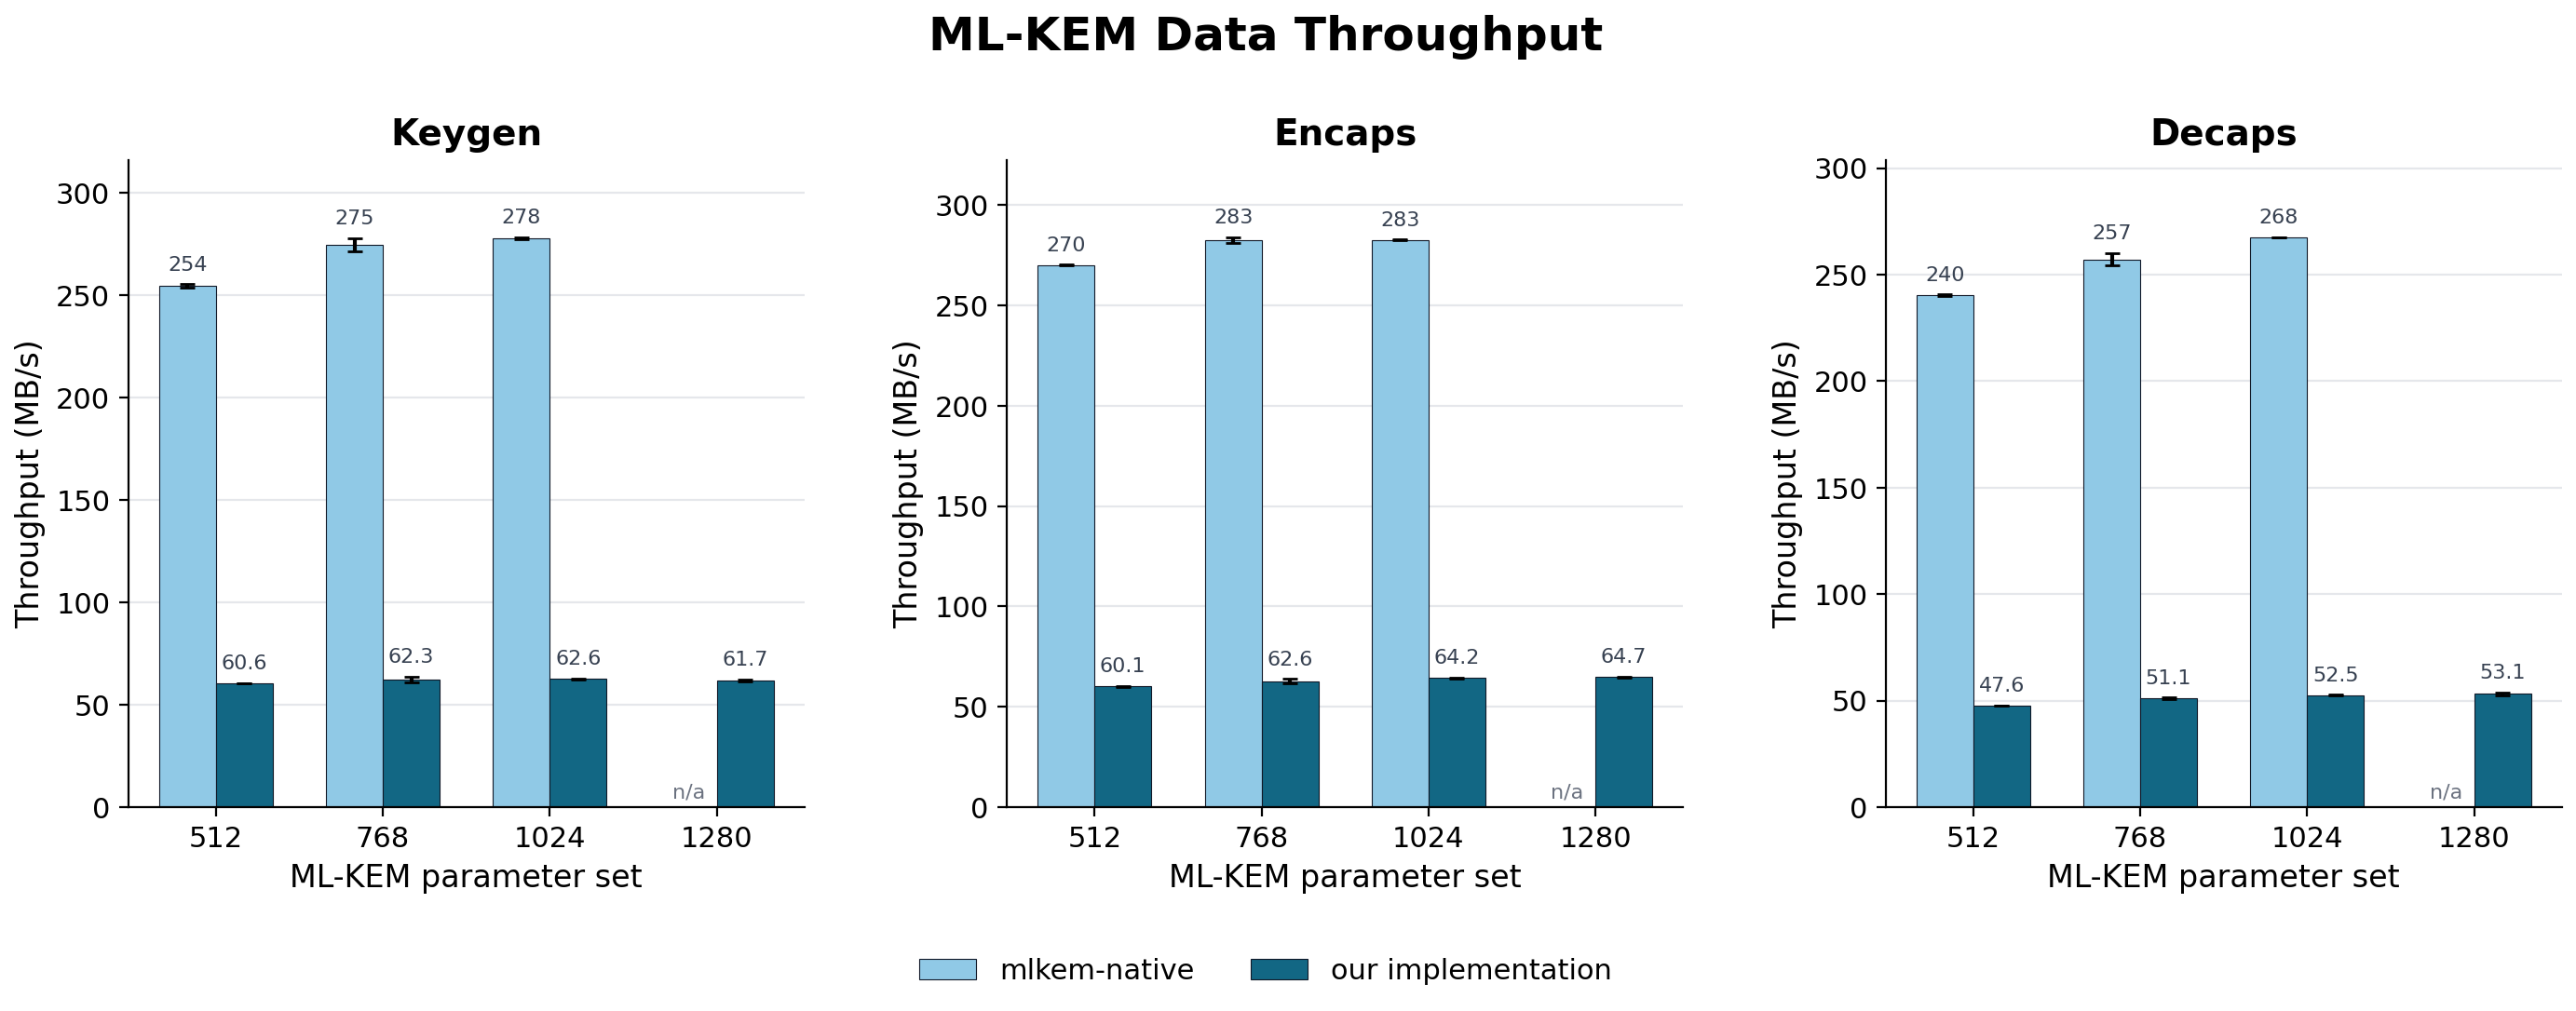
\includegraphics[width=1\textwidth]{images/mlkem-throughput-mbps.png}
    \caption{Approximate normalized internal-data throughput.}
    \label{fig:mlkem-mbps}
\end{figure}

Table~\ref{tab:normalized-throughput} verifies the values plotted in Figure~\ref{fig:mlkem-mbps}: the graph is obtained by multiplying each operations-per-second value in Table~\ref{tab:mlkem-benchmark} by the corresponding $D_{\mathrm{op}}(k)$ and dividing by $10^6$.

\subsection{Constant Timing Evaluation}

Welch $t$-tests in the style of dudect are used to search for timing distinguishers. For encapsulation, the deterministic internal hook allows the message to be classified as fixed or random without measuring operating-system randomness. For decapsulation, the two classes are valid ciphertexts and one-bit-modified invalid ciphertexts; this directly exercises the implicit rejection path. A separate key-generation scan fixes the main seed and varies the secret fallback value $z$.

\begin{table}[htbp]
    \centering
    \caption{Constant-timing test summary.}
    \label{tab:constant-timing}
    \begin{tabular}{l c c}
        \toprule
        \textbf{Test} & \textbf{Samples} & \textbf{Maximum $t$-statistic} \\
        \midrule
        Key generation $z$-scan & $1024 \times 128$ cases & $2.31$ \\
        Encapsulation             & $0.069$M samples        & $1.92$ \\
        Decapsulation             & $0.100$M samples        & $1.62$ \\
        \bottomrule
    \end{tabular}
\end{table}

The observed results did not indicate a strong timing distinguisher in these runs. As summarized in Table~\ref{tab:constant-timing}, all reported $t$-statistics remain below the conventional dudect warning threshold. These numbers provide empirical evidence that the measured paths do not exhibit a statistically significant timing difference under this test setup. They do not provide a formal constant-time guarantee.

\section{Discussion}

The implementation confirms the architectural point developed in the earlier chapters: ML-KEM is best understood as a layered construction. The module-lattice K-PKE core supplies a noisy but correct CPA-secure encryption mechanism; the control plane binds public keys, derives coins and shared secrets, and enforces implicit rejection; the public KEM API exposes only key generation, encapsulation, and decapsulation. This separation makes the design easier to test and reason about, and it matches the KEM abstraction used in modern protocols.

The main limitation of the implementation is performance. Without architecture-specific vectorization or assembly, polynomial multiplication, NTT operations, sampling, and hashing remain significantly slower than optimized native implementations. Even with this limitation, the implementation is sufficient for experimental evaluation and for demonstrating how the formal KEM construction is realized as executable software.
